\chapter{Clustering Techniques}
\label{chapter:clustering}

%Describe our basic assumption of function decomposition.
%Each subproblem should be composed of an observalbe uni-model.
We are interested in solving real-valued multimodal problems composed of observable unimodals.
Given the case, it is easier to solve an isolated unimodal within a subspace,
than tackling the complete search space with the multimodal problem.
Therefore, the first thing for solving a multimodal problem is to \textbf{identify} and \textbf{isolate}
the potential uni-modals within the given search space.

%We wish to identify these uni-models through clustering techniques. 
We tried to isolate potential \textit{fitness hills}, i.e. uni-modals,
by \textbf{clustering} the initial samples points,
and consider each cluster as a multi-dimension normal distribution.
Different clustering techniques are often applied to identify different characteristics of clusters.
Here we proposed a \textit{hierarchical clustering} techniques to identify \textit{fitness hills},
since we consider not only the density of the particles,
but also the fitness values of different search points.
Our basic assumption for the under lying uni-modal is a weighted normal distribution, 
since we need to take fitness into account instead of viewing each point with the same weight.
We tend to focus on the particles with better fitness,
than a dense cluster with less fitness. 
It is also easier to calculate the weighted mean vector and weighted covariance matrix in higher dimension. 

Later, we applied the \textbf{Minimum Description Length} (MDL) to reduce the number of clusters.
Although a complex Gaussian Mixture Modal is able to describe the sample distribution better,
we believe that a more compact model, in terms of information entropy, is the better choice 
when multiple models can describe the same distribution. 
This also allows us to define a more stable subspace for further searching.


\section{K-Means Clustering}
In this section, we first describe the K-Means clustering techniques and its limitation for identifying the fitness hills.
K-Means clustering aims to partition $n$ observation data points into $k$ clusters.
There are two main procedures for K-Means clustering: the \textit{assignment} step and the \textit{update} step.

During the \textit{assignment} step, an initial set of $k$ means positions are given.
Then, each data point is assigned to the cluster with the \textit{nearest mean}.
The assignment to the \textit{nearest mean} can be formally described 
as creating clusters whose mean yields the least within-cluster sum of squares (WCSS), i.e. the sum of squared Euclidean distance.
During the \textit{update} step, the new centroids of each new clusters are calculated and assigned as the new means.
This can be also be described as minimizing the WCSS.
The algorithm proceeds by alternating between these two steps until the means no longer change.
Since there only exists a finite states of partitions, the algorithm must converge to a local optimum.
However, different initial mean positions results in different clusters.

One of the main problem for using the K-Means clustering to identify \textit{fitness hills} is that
it considers only the \textit{spatial density} and does not utilize the fitness value of each particle.
Different sets of initial centers might result in different kinds of clusters.
Meanwhile, each cluster might be centering at a point that does not necessarily possess the best fitness in the neighborhood.
Therefore, the K-Means clustering often results in \textbf{unstable clusters} depending on initial conditions, and is highly sensitive to particle density.
Another common phenomenon for being sensitive to spatial density is that 
the points on the \textit{border of clusters} might belong to different clusters after each update.
This makes the clusters unstable and costs unnecessary evaluations and computation for redefining the borders of ROI after each update. 

The other problem for using the K-Means clustering is that one needs to \textbf{decide the number of clusters}.
Determining the number of clusters is also a highly studied subjects.
We breifly discuss three common estimation methods that we have tried, 
the \textit{silhouette coefficient}, the \textit{gap statistics} and the \textit{dip test} in the following paragraph.

The silhouette coefficient~\cite{Rousseeuw:1987:silhouettes} measures how cohesive an object is to its own cluster and how seperate it is to the other clusters. Ranging from -1 to 1, the silhouette coefficient with a higher value indicates it is more likely to belong to its own cluster.
The gap statistics~\cite{Tibshirani:2001:gap} compares the change in within-cluster dispersion with that of an reference null distribution.
It calculates the gap statistics for different number of clusters and select the one with the maximum gap statistics.
The Hartigans' dip test~\cite{Hartigan:1985:dip} uses the empirical cumulative distribution function (ECDF) to measure the maximum difference between multimodal samples and the unimodal samples. It calculates maximum deviation of the sample ECDF from the unimodal CDF and check if the difference is statistically significant.


We wish that as the algorithms proceed, particles should gather around the good solutions and gives a clear density signal.
However, they seldom identify a unimodal at the beginning.
It means that we need to add up more particles to meet the population size requirement for each clusters.
This increases the density in that specific region, and creates an artificial cluster that should not exist in the first place.

\begin{figure} 
\centering
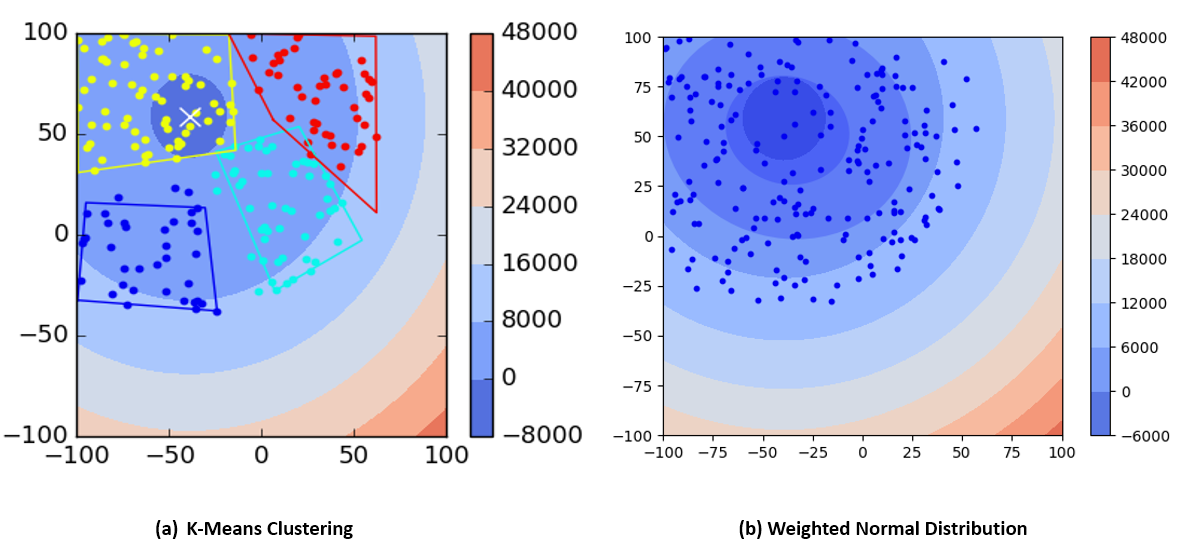
\includegraphics[width=\textwidth]{Clustering_comparison} 
\caption{Comparing K-Means clustering with weighted Gaussian Distribution on CEC2005 F1 Problem}\label{fig:Clustering_comparison}
\end{figure}

Figure~\ref{fig:Clustering_comparison} shows how K-Means fails to identify a unimodal and results in four clusters due to density.
A more preferable clustering result is shown on the right in Figure~\ref{fig:Clustering_comparison}.
We would like our clustering method to be capable of identifying the uni-modal 
and be able to center around the particle with the best fitness.

\begin{figure}
\centering
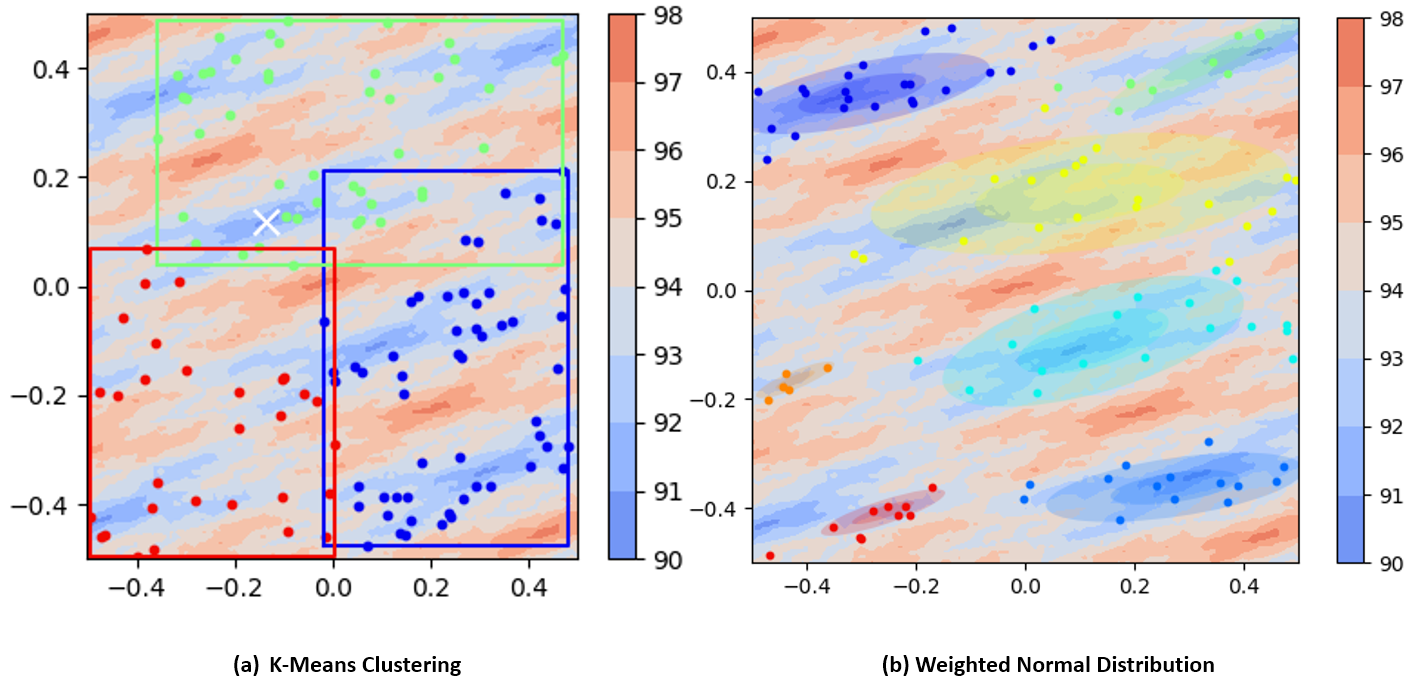
\includegraphics[width=\textwidth]{Clustering_comparison_F11}
\caption{Comparing K-Means clustering with weighted Gaussian Distribution on CEC2005 F11 Problem}\label{fig:Clustering_comparison_F11}
\end{figure}

Figure~\ref{fig:Clustering_comparison_F11} shows another example of how K-Means fails to identify the right multimodals.
Since K-Means only consider the density, it is hard to recognize the dense hills in the landscape. 
This initial clusters leads to more unnecassy evaluations for merging and reidentifying the hills.
However, we can see that on the right, our technique successfully recognize almost all the hills in the problem.
It also helps to locate the local optimum solutions approximately at the center.
This gives alot of advantage for the algorithms to search, since the task becomes exploiting a single hill.
Therefore, later we adopted the weighted normal distribution as the underlying model. 


\section{Heirarchical Clustering}\label{section:hierarchical}

Since we would like to recognize the \textit{fitness hills}, 
we modified the agglomerative clustering technique to create hierarchical clusters.
For a problem in $D$ dimension, we defined the neighborhood of a particle 
to be the $ 4 + \lfloor 3\log(D) \rfloor $ particles with the minimum Euclidean distance, including the particle itself.
Given the neighborhood of each particle, 
we create a directed graph by pointing each particle to the particle with the highest fitness in the neighborhood.
If a particle does not possess the best fitness in its neighborhood, it points toward the direction with the maximum gradient.
If it is the best particle in the neighborhood, it is very likely to be at the approximate location of local minimum.

We then create trees with the directed graph, 
where each tree represents a cluster with a potential fitness hill.
The best position within this cluster is indicated by the root node.  
This way, the fitness signal guides the construciton of clusters, 
so that this method is able to identify more \textit{fitness hills} than the K-Means clustering.
Moreover, we do not need to provide the estimate number of clusters, 
since the agglomerative clustering method \textit{intrinsically identifies hills} 
These characteristics solves some fundamental problems that we faced when using the K-Means clustering along with different number-of-clusters-estimation techniques.

\begin{figure}
\centering
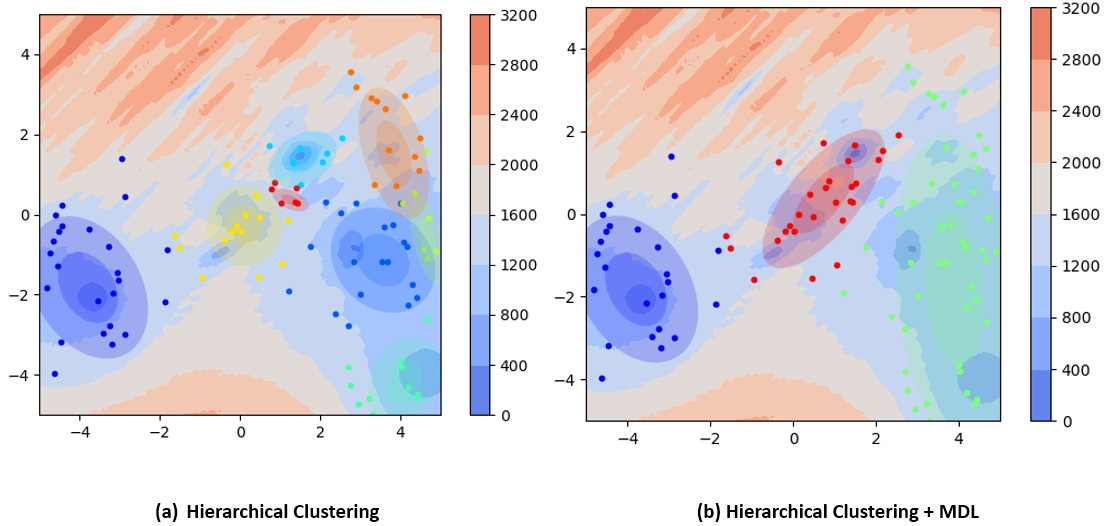
\includegraphics[width=\textwidth]{MDL_comparison_F19}
\caption{Before and after Minimal Description Length trimming on CEC2005 F19 Problem}\label{fig:MDL_comparison_F19}
\end{figure}

\begin{figure} 
\centering
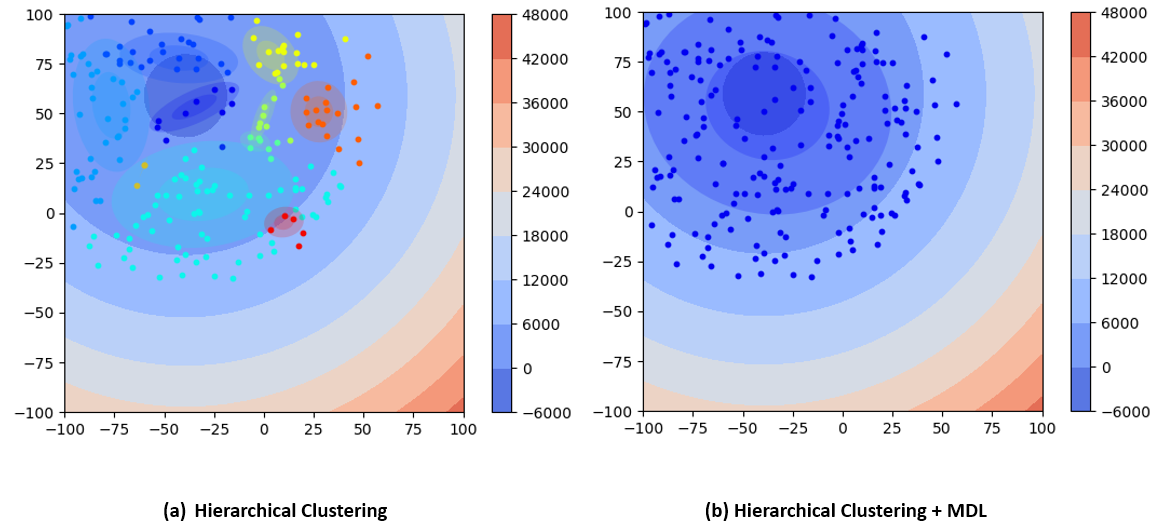
\includegraphics[width=\textwidth]{MDL_comparison}
\caption{Before and after Minimal Description Length trimming on CEC2005 F1 Problem}\label{fig:MDL_comparison}
\end{figure}

We can see that for a multimodal problem depicted in Figure~\ref{fig:MDL_comparison_F19}(a), 
the hierarchical clustering technique successfully identifies several fitness hills.
However, for the unimodal problem in Figure~\ref{fig:MDL_comparison}(a), 
the hierarchical clustering creates multiple ``ripples'' on the marginal area.
These clusters are created when the best particle is a bit further from the next best particle.
This indicates that the using the Euclidean distance as the distance metric is not suitable for problems with larger hills.

In order to solve this problem, we assume the underlying hills are composed of multivariate normal distribution.
Given the distribution and a sample position, we can use the \textit{Manhanoblis distance} to serve as a more expressive metric.
We would also like to trim down the number of clusters in the beginning, since we believe that the problems are composed of hierarchical hills.
We do not need to invest so much resources in so many regions during the initialization.
Reclustering after a few iterations shall give us a better signal about where to focus.


\section{Minimum Description Length} 
The Minimum Description Length (MDL) principle was introduced by Rissanen in 1978~\cite{Rissanen:1978:MDL}.
It adopts the idea of Occams's razor by selecting the codec that gives the shortest codelength of the data.
It provides a natural safeguard against overfitting, 
since it considers not only the goodness of the model, 
but also the complexity of the data to give the hypothesis.
Here we modified the MDL described in~\cite{Kyrgyzov:2007:KMDL} to help us determine the optimum number of clusters that provides the most efficient codes for the sample data.
The MDL considers both \textit{data description accuracy} and \textit{model description efficiency}.


\subsection{Data description accuracy}

Since we would like to take the fitness into account, we use the weighted Gaussian distribution as the underlying model.
For a cluster with $N$ particles, each particle $X_i$ has a rank $r_i$ between 1 and N (ties are broken randomly) that corresponds to the fitness.
The weight $\omega_i$ can be defined as:
\begin{equation}
\omega_i = \log(N+0.5) - \log(r_i)
\end{equation}

The mean $\mu$ and covariance matrix $\Sigma$ in a weighted Gaussian distribution $N$ can be denoted as:
\begin{equation}
\mu = \frac{1}{\sum_{i=1}^N \omega_i} \sum_{i = 1}^{N} \omega_i X_i
\end{equation}
\begin{equation}
\Sigma = \frac{1}{\sum_{i=1}^N \omega_i} \sum_{i = 1}^{N} \omega_i (X_i - \mu)^T (X_i - \mu)
\end{equation}


Let $X = \{X_1, X_2, ..., X_I\}$ denote the data set, composed of $I$ samples. 
Each sample is a $D$-dimensional vector $X_i = \{X_{i1}, ..., X_{iD}\}$.  
The class-probability of observing sample $X_i$ in class $j$, described by a parameter set $\Theta_j$, can be denoted as $P_j(X_i|\Theta_j)$.
The probability of observing the sample $X_i$ in a finite mixture model with $J$ components can be denoted as:
\begin{equation}
P(X_i|\Theta) = \sum_{j=1}^J \alpha_j P_j ( X_i | \Theta_j )
\end{equation}
\begin{equation}
\alpha_j = n_j / I
\end{equation}
where $\alpha_j$ is the prior probaility that $X_i$ belongs to the $j$-th model, 
and $n_j$ denotes the number of samples in cluster $j$.  

Therefore, the probability of observing sample $X_i$ in cluster $j$ can be further described by the $j$-th weighted Gaussain distribution:

\begin{equation}
P(X_i|\Theta_j) = N(X_i | \mu_j, \Sigma_j)
\end{equation}

With the assumption that the data instance $X_i$ are independently distributed, 
the joint data probability is the product of the individual instance probabilities:
\begin{equation}
P(X|\Theta) = \prod_{i=1}^{I} \sum_{j=1}^{J} \alpha_j P_j(X_i | \Theta_j)
\end{equation}



\subsection{Model description efficiency}
Although a more complex model can describe the data distribution better, 
we believe that a simpler model with approximately the same accuracy is better.
Therefore, the number of parameters that a model requires, is also considered in MDL.
The free parameters in the Gaussian mixture model are:
\begin{itemize}
\item $J-1$ paramters for $J$ weights $\alpha_j$, since $\sum \alpha_j = 1$
\item $D$ parameters for each mean $\mu_j$
\item $D(D+1)/2$ parameters for each covariance matrix $\Sigma_j$
\end{itemize}

Therefore, the total number of free parameters is
\begin{equation}
\mathbb{K} = J - 1 + J(D + D(D+1)/2) = J(D^2 + 3D + 2)/2 -1
\end{equation}


Combining the \textit{data description accuracy} and \textit{model description efficiency}, 
the MDL defined in~\cite{Rissanen:1984:Universal} is denoted as:
\begin{equation}
\min_{\mathbb{K}, \Theta} - \log (P(X|\Theta)) + \frac{1}{2}\mathbb{K}\log(I)
\end{equation}\label{equation:MDL}


\subsection{Trimming model with MDL}
As mentioned before, we need to solve the problem of having too many ``ripple'' clusters on the margin area.
Here we would like to use the MDL Equation to calculate model efficiency, and trim down unnecessary clusters.
Therefore, after identifying potential unimodals with hierarchical clustering in Section~\ref{section:hierarchical},
we use Equation~\ref{equation:MDL} to calculate model efficiency.
We created mutliple weighted Gaussian distribution according to the hierarchical clusters, 
as shown in Figure~\ref{fig:MDL_comparison}(a) and Figure~\ref{fig:MDL_comparison_F19}(a).
Then we try all combinations of merging two clusters and calculate the corresponding MDL.
Therefore, we compare the MDL score between the original hierarchical clusters and the new clusters with the minimal MDL score.
If the MDL score of the new model is smaller than the previous model, we repeat the same procedure and keep merging.
This trimming procedure terminates when there is only one cluster remain, or when the minimum MDL score of all possible new modals is larger than the MDL score of the previous model.
Then we get fewer yet still expressive clusters, 
shown in Figure~\ref{fig:MDL_comparison}(b) and Figure~\ref{fig:MDL_comparison_F19}(b).















